% !TEX TS-program = pdflatexmk
\documentclass[12pt]{amsart}

%\usepackage[parfill]{parskip}    % Activate to begin paragraphs with an empty line rather than an indent

\usepackage[margin=1in]{geometry}

\usepackage{amsmath,amssymb,amsthm,latexsym,graphicx}
\usepackage[normalem]{ulem}
\usepackage{setspace} %used for doublespacing, etc.
\usepackage{hyperref}
\usepackage[dvipsnames,usenames]{color}
\usepackage{fancyhdr}
\pagestyle{fancy}
	\renewcommand{\headrulewidth}{0.5pt} % and the line
	\headsep=1cm
	
\DeclareGraphicsRule{.tif}{png}{.png}{`convert #1 `dirname #1`/`basename #1 .tif`.png}

%Some useful environments.
\newtheorem{theorem}{Theorem}
\newtheorem{corollary}[theorem]{Corollary}
\newtheorem{conjecture}[theorem]{Conjecture}
\newtheorem{lemma}[theorem]{Lemma}
\newtheorem{proposition}[theorem]{Proposition}
\newtheorem{definition}[theorem]{Definition}
\newtheorem{example}[theorem]{Example}
\newtheorem{axiom}{Axiom}
\theoremstyle{remark}
\newtheorem{remark}{Remark}
\newtheorem*{exercise}{Exercise}%[section]

%Some shortcuts helpful for our assignments
\newcommand{\bx}{\begin{exercise}}
\newcommand{\ex}{\end{exercise}}

%Some useful shortcuts for our favorite sets of numbers.
%Note, you can use these WITHOUT entering math mode
\def\RR{\ensuremath{\mathbb R}} 
\def\NN{\ensuremath{\mathbb N}}
\def\ZZ{\ensuremath{\mathbb Z}}
\def\QQ{{\ensuremath\mathbb Q}}
\def\CC{\ensuremath{\mathbb C}}
\def\EE{{\ensuremath\mathbb E}}

%Some useful shortcuts for formatting lists
\newcommand{\bc}{\begin{center}}
\newcommand{\ec}{\end{center}}
\newcommand{\be}{\begin{enumerate}}
\newcommand{\ee}{\end{enumerate}}
\newcommand{\bi}{\begin{itemize}}
\newcommand{\ei}{\end{itemize}}

%Some useful shortcuts for formatting mathematical symbols
\newcommand{\ol}[1]{\overline{#1}}
\newcommand{\oimp}[1]{\overset{#1}{\iff}} %labeled iff symbol
\newcommand{\bv}[1]{\ensuremath{ \vec{\mathbf{#1}}} } %makes a vector.
\newcommand{\mc}[1]{\ensuremath{\mathcal{#1}}} %put something in caligraphic font
\newcommand{\normale}{\trianglelefteq}
\newcommand{\normal}{\triangleleft}

%Code for formatting the proofs a little nicer for submitted homework
\makeatletter
\renewenvironment{proof}[1][\proofname]{\par\doublespacing
  \pushQED{\qed}%
  \normalfont \topsep6\p@\@plus6\p@\relax
  \list{}{%
    \settowidth{\leftmargin}{\itshape\proofname:\hskip\labelsep}%
    \setlength{\labelwidth}{0pt}%
    \setlength{\itemindent}{-\leftmargin}%
  }%
  \item[\hskip\labelsep\itshape#1\@addpunct{:}]\ignorespaces
}{%
  \popQED\endlist\@endpefalse
  \singlespacing
}
\makeatother


%Commenting tools for the professor
\newcommand{\mpg}[1]{\marginpar{ #1}} %to put comments in margins
\usepackage{soul}
\definecolor{highlight}{rgb}{1,0.6,0.6}
\sethlcolor{highlight}
\newcommand{\hlm}[1]{\colorbox{highlight}{$\displaystyle #1$}}
\newtheoremstyle{mycomment}{\topsep}{-0in}{\small \itshape \sffamily}{}{\small \itshape\sffamily}{:}{.5em}{}
\theoremstyle{mycomment}
\newtheorem*{acomment}{\color{BrickRed}{Comment}}
\newcommand{\com}[1]{{\color{OliveGreen}\begin{acomment}{#1} %#2 \color{black} 
\end{acomment}\noindent}}
\newcommand{\red}[1]{{\color{BrickRed} #1}}
\newcommand{\blue}[1]{{\color{MidnightBlue}#1}}
\newcommand{\green}[1]{{\color{OliveGreen}#1}}
\newcommand{\mwrong}[2]{\red{\cancel{#1}}\green{#2}}
\newcommand{\wrong}[2]{\red{\sout{#1}}\green{#2}}
\definecolor{OliveGreen}{rgb}{.3,.5,.2}
\definecolor{MidnightBlue}{rgb}{.3,.4,.6}
\newcommand{\pts}[1]{\hfill\blue{{#1}/5}}

\chead{MATH 371}
\pagestyle{fancy}
%Modify these items:
\rhead{\emph{Christopher Munoz}}
\lhead{\emph{HW 8}}

\begin{document}

\thispagestyle{fancy}
%§12.1 1, 3, 7, 9, 12.
\section*{4.2}

\begin{exercise}[4.1]
Let $Y$ be a random variable with $p(y)$ given in the table below.
\begin{center}
\begin{tabular}{c|cccc}
$y$ & 1 & 2 & 3 & 4 \\
\hline
$p(y)$ & .4 & .3 & .2 & .1
\end{tabular}
\end{center}

\begin{enumerate}
    \item[(a)] Give the distribution function, $F(y)$. Be sure to specify the value of $F(y)$ for all $y$, $-\infty < y < \infty$.
\begin{proof}[Solution]
 $$F(y) = P(Y \leq y) = \begin{cases}
	0, & y < 1 \\
	0.4, & 1 \leq y < 2 \\
	0.7, & 2 \leq y < 3 \\
	0.9, & 3 \leq y < 4 \\
	1, & y \geq 4
	\end{cases}$$
\end{proof}
    \item[(b)] Sketch the distribution function given in part (a).
\begin{proof}[Solution]
 	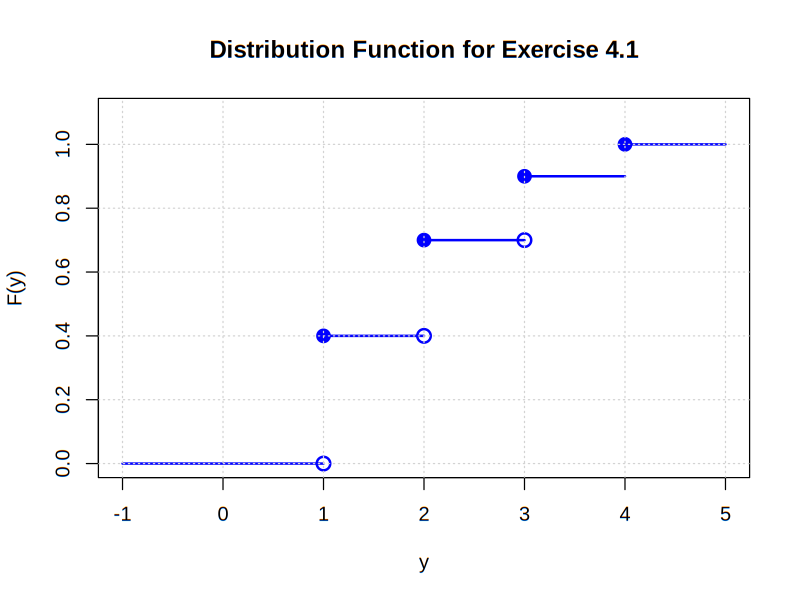
\includegraphics[width=0.7\textwidth]{exercise_4_1b.png}
\end{proof}
\end{enumerate} 
\end{exercise}

\begin{exercise}[4.3]
A Bernoulli random variable is one that assumes only two values, 0 and 1 with $p(1) = p$ and $p(0) = 1 - p \equiv q$.

\begin{enumerate}
    \item[(a)] Sketch the corresponding distribution function.
\begin{proof}[Solution]
 	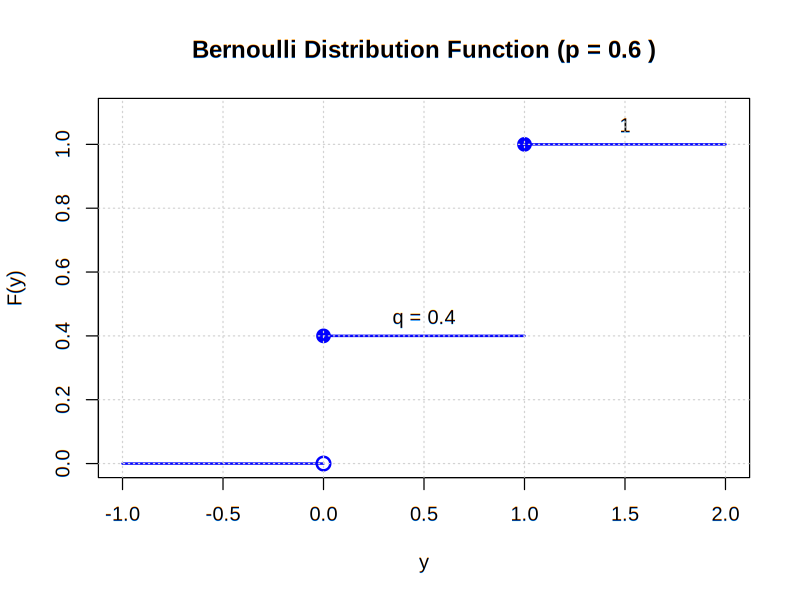
\includegraphics[width=0.7\textwidth]{exercise_4_3a.png}
\end{proof}
    \item[(b)] Show that this distribution function has the properties given in Theorem 4.1.
\begin{proof}[Solution]
 Theorem 4.1 properties:
	\begin{enumerate}
		\item $F(-\infty) = 0$: Yes, $\lim_{y \to -\infty} F(y) = 0$ 
		\item $F(\infty) = 1$: Yes, $\lim_{y \to \infty} F(y) = 1$ 
		\item $F$ is non-decreasing: $0 \leq q \leq 1$ since $q = 1-p$ and $0 \leq p \leq 1$ 
		\item $F$ is right-continuous: At each point, $F$ equals its right-hand limit 
	\end{enumerate}
\end{proof}
\end{enumerate} 
\end{exercise}

\begin{exercise}[4.5]
Suppose that $Y$ is a random variable that takes on only integer values $1, 2, \ldots$ and has distribution function $F(y)$. Show that the probability function $p(y) = P(Y = y)$ is given by
$$p(y) = \begin{cases}
F(1), & y = 1, \\
F(y) - F(y-1), & y = 2, 3, \ldots
\end{cases}$$

\begin{proof}[Solution]
 For $y = 1$: $P(Y = 1) = P(Y \leq 1) = F(1)$ since $Y$ takes integer values $\geq 1$.
	
	For $y \geq 2$:
	\begin{align*}
		P(Y = y) &= P(Y \leq y) - P(Y \leq y-1) \\
		&= F(y) - F(y-1)
  \end{align*}
\end{proof}
\end{exercise}

\begin{exercise}[4.7]
Let $Y$ be a binomial random variable with $n = 10$ and $p = 0.2$.

\begin{enumerate}
    \item[(a)] Use Table 1, Appendix 3, to obtain $P(2 < Y < 5)$ and $P(2 \leq Y < 5)$. Are the probabilities that $Y$ falls in the intervals $(2, 5)$ and $[2, 5)$ equal? Why or why not?
\begin{proof}[Solution]
 $P(2 < Y < 5) = P(Y = 3) + P(Y = 4) = P(Y \leq 4) - P(Y \leq 2) = 0.967 - 0.678 = 0.289$
	
	$P(2 \leq Y < 5) = P(Y = 2) + P(Y = 3) + P(Y = 4) = P(Y \leq 4) - P(Y \leq 1) = 0.967 - 0.376 = 0.591$
	
	not equal because $Y$ is discrete. For discrete variables, $(2,5)$ excludes 2 while $[2,5)$ includes 2.
\end{proof}
    \item[(b)] Use Table 1, Appendix 3, to obtain $P(2 < Y \leq 5)$ and $P(2 \leq Y \leq 5)$. Are these two probabilities equal? Why or why not?
\begin{proof}[Solution]
 $P(2 < Y \leq 5) = P(Y = 3) + P(Y = 4) + P(Y = 5) = P(Y \leq 5) - P(Y \leq 2) = 0.994 - 0.678 = 0.316$
	
	$P(2 \leq Y \leq 5) = P(Y \leq 5) - P(Y \leq 1) = 0.994 - 0.376 = 0.618$
	
	not equal because including/excluding $Y = 2$ makes a difference for discrete variables.
\end{proof}
    \item[(c)] Earlier in this section, we argued that if $Y$ is continuous and $a < b$, then $P(a < Y < b) = P(a \leq Y < b)$. Does the result in part (a) contradict this claim? Why?
\begin{proof}[Solution]
 no this does not contradict the claim. The claim is specifically for continuous random variables, where $P(Y = a) = 0$ for any specific value $a$. Here, $Y$ is \textbf{discrete}, so $P(Y = 2) \neq 0$, and therefore the inclusion/exclusion of endpoints matters.
\end{proof}
\end{enumerate} 
\end{exercise}

\begin{exercise}[4.9]
A random variable $Y$ has the following distribution function:
$$F(y) = P(Y \leq y) = \begin{cases}
0, & \text{for } y < 2, \\
1/8, & \text{for } 2 \leq y < 2.5, \\
3/16, & \text{for } 2.5 \leq y < 4, \\
1/2, & \text{for } 4 \leq y < 5.5, \\
5/8, & \text{for } 5.5 \leq y < 6, \\
11/16, & \text{for } 6 \leq y < 7, \\
1, & \text{for } y \geq 7.
\end{cases}$$

\begin{enumerate}
    \item[(a)] Is $Y$ a continuous or discrete random variable? Why?
\begin{proof}[Solution]
 
\end{proof}
    \item[(b)] What values of $Y$ are assigned positive probabilities?
\begin{proof}[Solution]
 
\end{proof}
    \item[(c)] Find the probability function for $Y$.
\begin{proof}[Solution]
 
\end{proof}
    \item[(d)] What is the median, $\phi_{.5}$, of $Y$?
\begin{proof}[Solution]
 
\end{proof}
\end{enumerate} 
\end{exercise}

\begin{exercise}[4.11]
Suppose that $Y$ possesses the density function
$$f(y) = \begin{cases}
cy, & 0 \leq y \leq 2, \\
0, & \text{elsewhere}.
\end{cases}$$

\begin{enumerate}
    \item[(a)] Find the value of $c$ that makes $f(y)$ a probability density function.
\begin{proof}[Solution]
 For $f(y)$ to be a pdf: $\int_{-\infty}^{\infty} f(y) dy = 1$
	
	$$\int_0^2 cy \, dy = c \left[\frac{y^2}{2}\right]_0^2 = c \cdot 2 = 1$$
	
	Therefore, $c = 1/2$.
\end{proof}
    \item[(b)] Find $F(y)$.
\begin{proof}[Solution]
 For $y < 0$: $F(y) = 0$
	
	For $0 \leq y \leq 2$:
	$$F(y) = \int_0^y \frac{1}{2}t \, dt = \frac{1}{2} \cdot \frac{y^2}{2} = \frac{y^2}{4}$$
	
	For $y > 2$: $F(y) = 1$
	
	$$F(y) = \begin{cases}
	0, & y < 0 \\
	y^2/4, & 0 \leq y \leq 2 \\
	1, & y > 2
	\end{cases}$$
\end{proof}
    \item[(c)] Graph $f(y)$ and $F(y)$.
\begin{proof}[Solution]
 	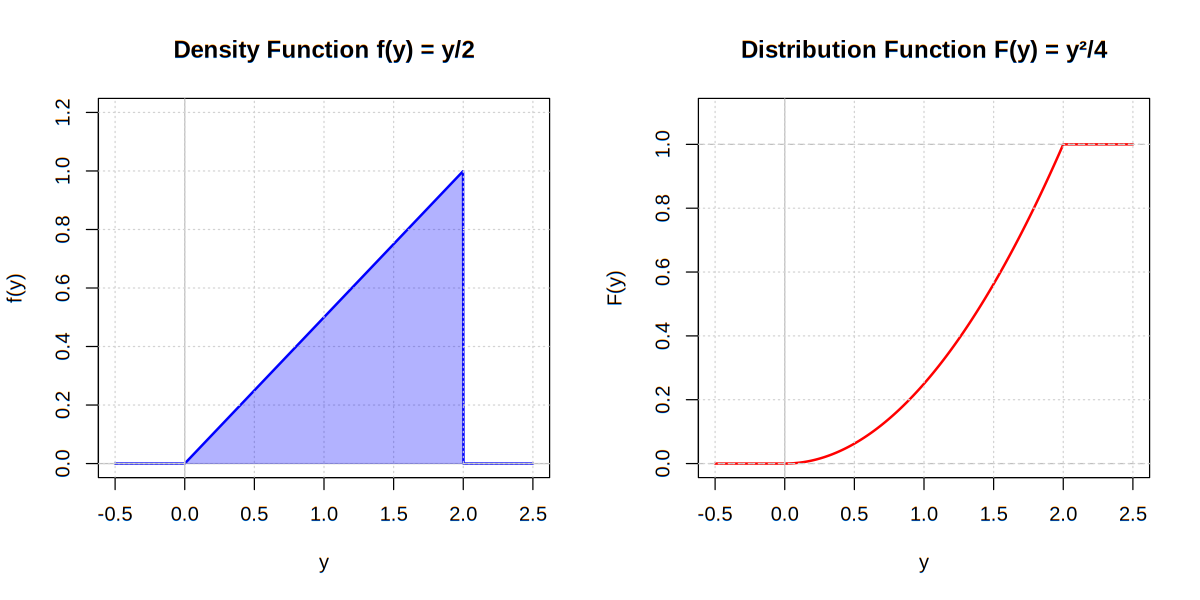
\includegraphics[width=0.7\textwidth]{exercise_4_11c.png}
\end{proof}
    \item[(d)] Use $F(y)$ to find $P(1 \leq Y \leq 2)$.
\begin{proof}[Solution]
 $$P(1 \leq Y \leq 2) = F(2) - F(1) = 1 - \frac{1}{4} = \frac{3}{4}$$
\end{proof}
    \item[(e)] Use $f(y)$ and geometry to find $P(1 \leq Y \leq 2)$.
\begin{proof}[Solution]
 	$$P(1 \leq Y \leq 2) = \int_1^2 \frac{y}{2} dy = \frac{1}{2} \left[\frac{y^2}{2}\right]_1^2 = \frac{1}{4}(4 - 1) = \frac{3}{4}$$
	
	Geometrically, this is the area of a trapezoid with parallel sides $f(1) = 1/2$ and $f(2) = 1$, and height 1:
	$$\text{Area} = \frac{1}{2}(1/2 + 1)(1) = \frac{3}{4}$$
\end{proof}
\end{enumerate} 
\end{exercise}

\begin{exercise}[4.13]
A supplier of kerosene has a 150-gallon tank that is filled at the beginning of each week. His weekly demand shows a relative frequency behavior that increases steadily up to 100 gallons and then levels off between 100 and 150 gallons. If $Y$ denotes weekly demand in hundreds of gallons, the relative frequency of demand can be modeled by
$$f(y) = \begin{cases}
y, & 0 \leq y \leq 1, \\
1, & 1 < y \leq 1.5, \\
0, & \text{elsewhere}.
\end{cases}$$

\begin{enumerate}
    \item[(a)] Find $F(y)$.
\begin{proof}[Solution]
 For $y < 0$: $F(y) = 0$
	
	For $0 \leq y \leq 1$: $F(y) = \int_0^y t \, dt = \frac{y^2}{2}$
	
	For $1 < y \leq 1.5$: $F(y) = \int_0^1 t \, dt + \int_1^y 1 \, dt = \frac{1}{2} + (y - 1) = y - \frac{1}{2}$
  For $y > 1.5$: $F(y) = 1$
  \begin{align*}
	F(y) = \begin{cases}
	0, & y < 0 \\
	y^2/2, & 0 \leq y \leq 1 \\
	y - 1/2, & 1 < y \leq 1.5 \\
	1, & y > 1.5
	\end{cases}
\end{align*}
\end{proof}
    \item[(b)] Find $P(0 \leq Y \leq 0.5)$.
\begin{proof}[Solution]
 	$$P(0 \leq Y \leq 0.5) = F(0.5) - F(0) = \frac{(0.5)^2}{2} - 0 = \frac{0.25}{2} = 0.125$$
\end{proof}
    \item[(c)] Find $P(0.5 \leq Y \leq 1.2)$.
\begin{proof}[Solution]
 	$$P(0.5 \leq Y \leq 1.2) = F(1.2) - F(0.5) = \left(1.2 - \frac{1}{2}\right) - \frac{(0.5)^2}{2} = 0.7 - 0.125 = 0.575$$
\end{proof}
\end{enumerate} 
\end{exercise}

\begin{exercise}[4.17]
The length of time required by students to complete a one-hour exam is a random variable with a density function given by
$$f(y) = \begin{cases}
cy^2 + y, & 0 \leq y \leq 1, \\
0, & \text{elsewhere}.
\end{cases}$$

\begin{enumerate}
    \item[(a)] Find $c$.
\begin{proof}[Solution]
 	For $f(y)$ to be a pdf: $\int_{-\infty}^{\infty} f(y) dy = 1$
	
	$$\int_0^1 (cy^2 + y) dy = \left[\frac{cy^3}{3} + \frac{y^2}{2}\right]_0^1 = \frac{c}{3} + \frac{1}{2} = 1$$
	
	$$\frac{c}{3} = \frac{1}{2} \implies c = \frac{3}{2}$$
\end{proof}
    \item[(b)] Find $F(y)$.
\begin{proof}[Solution]
For $y < 0$: $F(y) = 0$
	
	For $0 \leq y \leq 1$:
	$$F(y) = \int_0^y \left(\frac{3}{2}t^2 + t\right) dt = \left[\frac{t^3}{2} + \frac{t^2}{2}\right]_0^y = \frac{y^3}{2} + \frac{y^2}{2} = \frac{y^2(y+1)}{2}$$
	
	For $y > 1$: $F(y) = 1$
	
	$$F(y) = \begin{cases}
	0, & y < 0 \\
	\frac{y^2(y+1)}{2}, & 0 \leq y \leq 1 \\
	1, & y > 1
	\end{cases}$$
\end{proof}
    \item[(c)] Graph $f(y)$ and $F(y)$.
\begin{proof}[Solution]
 	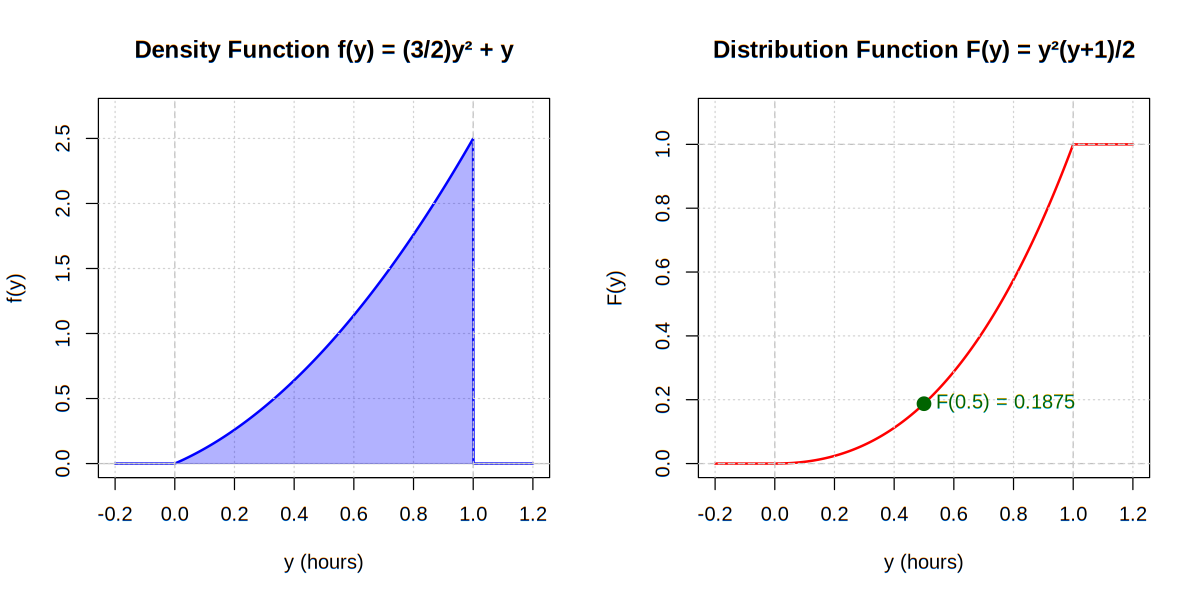
\includegraphics[width=0.7\textwidth]{exercise_4_17c.png}
\end{proof}
    \item[(d)] Use $F(y)$ in part (b) to find $F(-1)$, $F(0)$, and $F(1)$.
\begin{proof}[Solution]
 	$$F(-1) = 0$$
	$$F(0) = 0$$
	$$F(1) = \frac{1^2(1+1)}{2} = 1$$
\end{proof}
    \item[(e)] Find the probability that a randomly selected student will finish in less than half an hour.
\begin{proof}[Solution]
 	$$P(Y < 0.5) = F(0.5) = \frac{(0.5)^2(0.5+1)}{2} = \frac{0.25 \cdot 1.5}{2} = \frac{0.375}{2} = 0.1875$$
\end{proof}
    \item[(f)] Given that a particular student needs at least 15 minutes to complete the exam, find the probability that she will require at least 30 minutes to finish.
\begin{proof}[Solution]
 15 minutes = 0.25 hours, 30 minutes = 0.5 hours
	
	$$P(Y \geq 0.5 | Y \geq 0.25) = \frac{P(Y \geq 0.5)}{P(Y \geq 0.25)} = \frac{1 - F(0.5)}{1 - F(0.25)}$$
	
	$$F(0.25) = \frac{(0.25)^2(1.25)}{2} = \frac{0.078125}{2} = 0.0390625$$
	
	$$P(Y \geq 0.5 | Y \geq 0.25) = \frac{1 - 0.1875}{1 - 0.0390625} = \frac{0.8125}{0.9609375} \approx 0.846$$
\end{proof}
\end{enumerate} 
\end{exercise}

\begin{exercise}[4.19]
Let the distribution function of a random variable $Y$ be
$$F(y) = \begin{cases}
0, & y \leq 0, \\
\frac{y}{8}, & 0 < y < 2, \\
\frac{y^2}{16}, & 2 \leq y < 4, \\
1, & y \geq 4.
\end{cases}$$

\begin{enumerate}
    \item[(a)] Find the density function of $Y$.
\begin{proof}[Solution]
	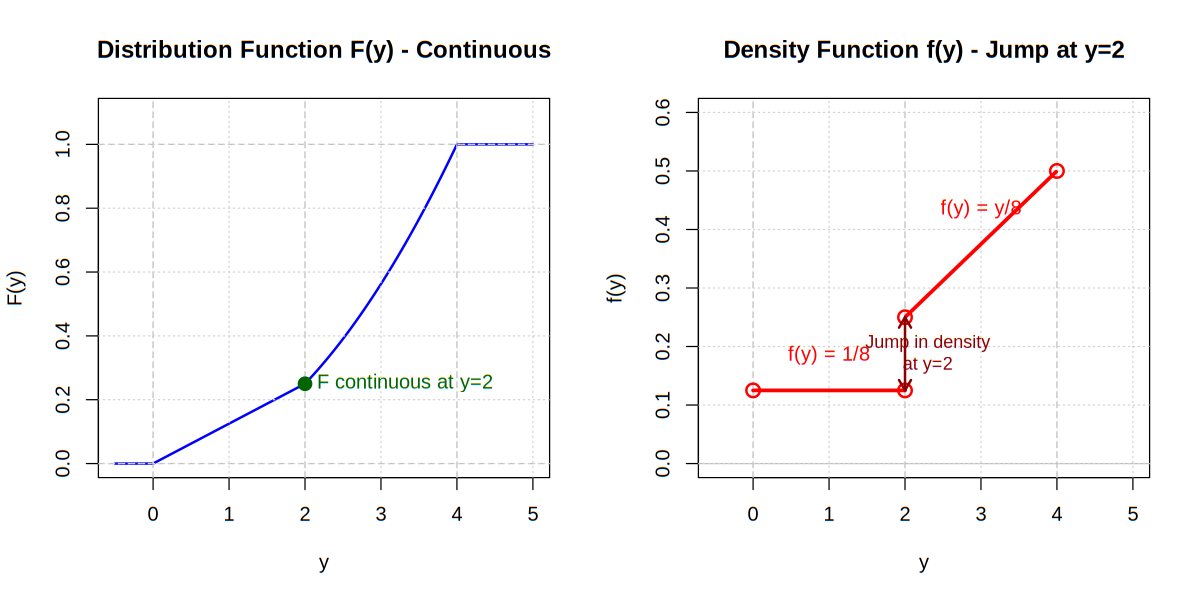
\includegraphics[width=0.7\textwidth]{exercise_4_19.png}
\end{proof}
   \item[(b)] Find $P(1 \leq Y \leq 3)$.
\begin{proof}[Solution]
$$P(1 \leq Y \leq 3) = F(3) - F(1) = \frac{3^2}{16} - \frac{1}{8} = \frac{9}{16} - \frac{2}{16} = \frac{7}{16}$$
\end{proof}

    \item[(c)] Find $P(Y \geq 1.5)$.
\begin{proof}[Solution]
$$P(Y \geq 1.5) = 1 - F(1.5) = 1 - \frac{1.5}{8} = 1 - \frac{3}{16} = \frac{13}{16}$$
\end{proof}

    \item[(d)] Find $P(Y \geq 1 \mid Y \leq 3)$.
\begin{proof}[Solution]
$$P(Y \geq 1 | Y \leq 3) = \frac{P(1 \leq Y \leq 3)}{P(Y \leq 3)} = \frac{F(3) - F(1)}{F(3)} = \frac{9/16 - 1/8}{9/16} = \frac{7/16}{9/16} = \frac{7}{9}$$
\end{proof}

\end{enumerate}

\end{exercise}
\section*{4.3}
\begin{exercise}[4.21]
If, as in Exercise 4.17, $Y$ has density function
$$f(y) = \begin{cases}
\frac{3}{2}y^2 + y, & 0 \leq y \leq 1, \\
0, & \text{elsewhere},
\end{cases}$$
find the mean and variance of $Y$.

\begin{proof}[Solution]
\textbf{Mean:}
\begin{align*}
E(Y) &= \int_0^1 y \left(\frac{3}{2}y^2 + y\right) dy = \int_0^1 \left(\frac{3}{2}y^3 + y^2\right) dy \\
&= \left[\frac{3}{8}y^4 + \frac{1}{3}y^3\right]_0^1 = \frac{3}{8} + \frac{1}{3} = \frac{9 + 8}{24} = \frac{17}{24}
\end{align*}

\textbf{Variance:} First find $E(Y^2)$:
\begin{align*}
E(Y^2) &= \int_0^1 y^2 \left(\frac{3}{2}y^2 + y\right) dy = \int_0^1 \left(\frac{3}{2}y^4 + y^3\right) dy \\
&= \left[\frac{3}{10}y^5 + \frac{1}{4}y^4\right]_0^1 = \frac{3}{10} + \frac{1}{4} = \frac{6 + 5}{20} = \frac{11}{20}
\end{align*}

\begin{align*}
V(Y) &= E(Y^2) - [E(Y)]^2 = \frac{11}{20} - \left(\frac{17}{24}\right)^2 \\
&= \frac{11}{20} - \frac{289}{576} = \frac{317.6 - 289}{576} = \frac{28.6}{576} = \frac{143}{2880} \approx 0.0497
\end{align*}

\end{proof}
\end{exercise}
\begin{exercise}[4.25]
If, as in Exercise 4.19, $Y$ has distribution function
$$F(y) = \begin{cases}
0, & y \leq 0, \\
\frac{y}{8}, & 0 < y < 2, \\
\frac{y^2}{16}, & 2 \leq y < 4, \\
1, & y \geq 4,
\end{cases}$$
find the mean and variance of $Y$.

\begin{proof}[Solution]
From Exercise 4.19(a), the density function is:
$$f(y) = \begin{cases}
\frac{1}{8}, & 0 < y < 2 \\
\frac{y}{8}, & 2 < y < 4 \\
0, & \text{otherwise}
\end{cases}$$

\textbf{Mean:}
\begin{align*}
E(Y) &= \int_0^2 y \cdot \frac{1}{8} dy + \int_2^4 y \cdot \frac{y}{8} dy \\
&= \frac{1}{8}\left[\frac{y^2}{2}\right]_0^2 + \frac{1}{8}\int_2^4 y^2 dy \\
&= \frac{1}{8} \cdot 2 + \frac{1}{8}\left[\frac{y^3}{3}\right]_2^4 \\
&= \frac{1}{4} + \frac{1}{8} \cdot \frac{64 - 8}{3} = \frac{1}{4} + \frac{56}{24} = \frac{1}{4} + \frac{7}{3} \\
&= \frac{3 + 28}{12} = \frac{31}{12}
\end{align*}

\textbf{Variance:} First find $E(Y^2)$:
\begin{align*}
E(Y^2) &= \int_0^2 y^2 \cdot \frac{1}{8} dy + \int_2^4 y^2 \cdot \frac{y}{8} dy \\
&= \frac{1}{8}\left[\frac{y^3}{3}\right]_0^2 + \frac{1}{8}\int_2^4 y^3 dy \\
&= \frac{1}{8} \cdot \frac{8}{3} + \frac{1}{8}\left[\frac{y^4}{4}\right]_2^4 \\
&= \frac{1}{3} + \frac{1}{8} \cdot \frac{256 - 16}{4} = \frac{1}{3} + \frac{240}{32} = \frac{1}{3} + \frac{15}{2} \\
&= \frac{2 + 45}{6} = \frac{47}{6}
\end{align*}

\begin{align*}
V(Y) &= E(Y^2) - [E(Y)]^2 = \frac{47}{6} - \left(\frac{31}{12}\right)^2 \\
&= \frac{47}{6} - \frac{961}{144} = \frac{1128 - 961}{144} = \frac{167}{144}
\end{align*}
\end{proof}
\end{exercise}
\begin{exercise}[4.26]
If $Y$ is a continuous random variable with mean $\mu$ and variance $\sigma^2$ and $a$ and $b$ are constants, use Theorem 4.5 to prove the following:

\begin{enumerate}
    \item[(a)] $E(aY + b) = aE(Y) + b = a\mu + b$.
\begin{proof}[Solution]
By Theorem 4.5:
\begin{align*}
E(aY + b) &= \int_{-\infty}^{\infty} (ay + b)f(y) dy \\
&= a\int_{-\infty}^{\infty} y f(y) dy + b\int_{-\infty}^{\infty} f(y) dy \\
&= aE(Y) + b(1) = a\mu + b
\end{align*}
\end{proof}

    \item[(b)] $V(aY + b) = a^2V(Y) = a^2\sigma^2$.
\begin{proof}[Solution]
\begin{align*}
V(aY + b) &= E[(aY + b)^2] - [E(aY + b)]^2 \\
&= E[a^2Y^2 + 2abY + b^2] - (a\mu + b)^2 \\
&= a^2E(Y^2) + 2abE(Y) + b^2 - a^2\mu^2 - 2ab\mu - b^2 \\
&= a^2E(Y^2) + 2ab\mu + b^2 - a^2\mu^2 - 2ab\mu - b^2 \\
&= a^2[E(Y^2) - \mu^2] = a^2V(Y) = a^2\sigma^2
\end{align*}
\end{proof}
\end{enumerate}
\end{exercise}
\begin{exercise}[4.27]
For certain ore samples, the proportion $Y$ of impurities per sample is a random variable with density function given in Exercise 4.21. The dollar value of each sample is $W = 5 - .5Y$. Find the mean and variance of $W$.

\begin{proof}[Solution]
From Exercise 4.21: $E(Y) = \frac{17}{24}$ and $V(Y) = \frac{139}{2880}$

Using Exercise 4.26 with $a = -0.5$ and $b = 5$:

\textbf{Mean:}
$$E(W) = E(5 - 0.5Y) = 5 - 0.5E(Y) = 5 - 0.5 \cdot \frac{17}{24} = 5 - \frac{17}{48} = \frac{240 - 17}{48} = \frac{223}{48}$$

\textbf{Variance:}
$$V(W) = V(5 - 0.5Y) = (-0.5)^2 V(Y) = 0.25 \cdot \frac{139}{2880} = \frac{139}{11520}$$
\end{proof}
\end{exercise}
\begin{exercise}[4.30]
The proportion of time $Y$ that an industrial robot is in operation during a 40-hour week is a random variable with probability density function
$$f(y) = \begin{cases}
2y, & 0 \leq y \leq 1, \\
0, & \text{elsewhere}.
\end{cases}$$

\begin{enumerate}
    \item[(a)] Find $E(Y)$ and $V(Y)$.
\begin{proof}[Solution]
\textbf{Mean:}
$$E(Y) = \int_0^1 y(2y) dy = 2\int_0^1 y^2 dy = 2\left[\frac{y^3}{3}\right]_0^1 = \frac{2}{3}$$

\textbf{Second moment:}
$$E(Y^2) = \int_0^1 y^2(2y) dy = 2\int_0^1 y^3 dy = 2\left[\frac{y^4}{4}\right]_0^1 = \frac{1}{2}$$

\textbf{Variance:}
$$V(Y) = E(Y^2) - [E(Y)]^2 = \frac{1}{2} - \left(\frac{2}{3}\right)^2 = \frac{1}{2} - \frac{4}{9} = \frac{9 - 8}{18} = \frac{1}{18}$$
\end{proof}

    \item[(b)] For the robot under study, the profit $X$ for a week is given by $X = 200Y - 60$. Find $E(X)$ and $V(X)$.
\begin{proof}[Solution]
$$E(X) = E(200Y - 60) = 200E(Y) - 60 = 200 \cdot \frac{2}{3} - 60 = \frac{400}{3} - 60 = \frac{220}{3} \approx 73.33$$

$$V(X) = V(200Y - 60) = 200^2 V(Y) = 40000 \cdot \frac{1}{18} = \frac{20000}{9}$$
\end{proof}

    \item[(c)] Find an interval in which the profit should lie for at least 75\% of the weeks that the robot is in use.
\begin{proof}[Solution]
Using Tchebysheff's theorem: $P(|X - \mu| < k\sigma) \geq 1 - \frac{1}{k^2}$

We want $1 - \frac{1}{k^2} = 0.75$, so $k = 2$.

$\mu_X = \frac{220}{3} \approx 73.33$ and $\sigma_X = \sqrt{\frac{20000}{9}} = \frac{100\sqrt{2}}{3} \approx 47.14$

The interval is:
$$\mu_X \pm 2\sigma_X = \frac{220}{3} \pm \frac{200\sqrt{2}}{3} \approx (73.33 - 94.28, 73.33 + 94.28) = (-20.95, 167.62)$$
\end{proof}
\end{enumerate}
\end{exercise}
\begin{exercise}[4.33]
Daily total solar radiation for a specified location in Florida in October has probability density function given by
$$f(y) = \begin{cases}
\frac{3}{32}(y - 2)(6 - y), & 2 \leq y \leq 6, \\
0, & \text{elsewhere},
\end{cases}$$
with measurements in hundreds of calories. Find the expected daily solar radiation for October.

\begin{proof}[Solution]
Expand: $f(y) = \frac{3}{32}(-y^2 + 8y - 12)$

\begin{align*}
E(Y) &= \int_2^6 y \cdot \frac{3}{32}(-y^2 + 8y - 12) dy \\
&= \frac{3}{32}\int_2^6 (-y^3 + 8y^2 - 12y) dy \\
&= \frac{3}{32}\left[-\frac{y^4}{4} + \frac{8y^3}{3} - 6y^2\right]_2^6 \\
&= \frac{3}{32}\left[\left(-324 + 576 - 216\right) - \left(-4 + \frac{64}{3} - 24\right)\right] \\
&= \frac{3}{32}\left[36 - \left(\frac{64}{3} - 28\right)\right] = \frac{3}{32} \cdot \frac{128}{3} = 4
\end{align*}

Expected daily solar radiation is 400 calories.
\end{proof}
\end{exercise}
\begin{exercise}[4.35]
If $Y$ is a continuous random variable such that $E[(Y - a)^2] < \infty$ for all $a$, show that $E[(Y - a)^2]$ is minimized when $a = E(Y)$. [Hint: $E[(Y - a)^2] = E(\{[Y - E(Y)] + [E(Y) - a]\}^2)$.]

\begin{proof}[Solution]
Let $\mu = E(Y)$. Following the hint:
\begin{align*}
E[(Y - a)^2] &= E[\{(Y - \mu) + (\mu - a)\}^2] \\
&= E[(Y - \mu)^2 + 2(Y - \mu)(\mu - a) + (\mu - a)^2] \\
&= E[(Y - \mu)^2] + 2(\mu - a)E(Y - \mu) + (\mu - a)^2 \\
&= V(Y) + 2(\mu - a)(0) + (\mu - a)^2 \\
&= V(Y) + (\mu - a)^2
\end{align*}

Since $V(Y) \geq 0$ is constant, $E[(Y - a)^2]$ is minimized when $(\mu - a)^2 = 0$, i.e., when $a = \mu = E(Y)$.

\end{proof}
\end{exercise}
\section*{4.4}
\begin{exercise}[4.39]
If a parachutist lands at a random point on a line between markers A and B, find the probability that she is closer to A than to B. Find the probability that her distance to A is more than three times her distance to B.

\begin{proof}[Solution]
Let the distance from A to B be normalized to the interval $(0, 1)$. Let $Y$ be the landing position, so $Y \sim \text{Uniform}(0, 1)$.

\textbf{Part 1: Closer to A than to B}

Closer to A means $Y < 0.5$ (left of midpoint).
$$P(Y < 0.5) = 0.5$$

\textbf{Part 2: Distance to A more than 3 times distance to B}

Distance to A: $Y$. Distance to B: $1 - Y$.

We want $Y > 3(1 - Y)$:
$$Y > 3 - 3Y \implies 4Y > 3 \implies Y > \frac{3}{4}$$

$$P\left(Y > \frac{3}{4}\right) = 1 - \frac{3}{4} = \frac{1}{4}$$
\end{proof}
\end{exercise}

\begin{exercise}[4.44]
The change in depth of a river from one day to the next, measured (in feet) at a specific location, is a random variable $Y$ with the following density function:
$$f(y) = \begin{cases}
k, & -2 \leq y \leq 2 \\
0, & \text{elsewhere}.
\end{cases}$$

\begin{enumerate}
    \item[(a)] Determine the value of $k$.
\begin{proof}[Solution]
For a valid pdf: $\int_{-\infty}^{\infty} f(y) dy = 1$

$$\int_{-2}^{2} k \, dy = k[y]_{-2}^{2} = k(2 - (-2)) = 4k = 1$$

$$k = \frac{1}{4}$$
\end{proof}

    \item[(b)] Obtain the distribution function for $Y$.
\begin{proof}[Solution]
For $y < -2$: $F(y) = 0$

For $-2 \leq y \leq 2$:
$$F(y) = \int_{-2}^{y} \frac{1}{4} dt = \frac{1}{4}[t]_{-2}^{y} = \frac{1}{4}(y + 2) = \frac{y + 2}{4}$$

For $y > 2$: $F(y) = 1$

$$F(y) = \begin{cases}
0, & y < -2 \\
\frac{y + 2}{4}, & -2 \leq y \leq 2 \\
1, & y > 2
\end{cases}$$
\end{proof}
\end{enumerate}
\end{exercise}
\begin{exercise}[4.45]
Upon studying low bids for shipping contracts, a microcomputer manufacturing company finds that intrastate contracts have low bids that are uniformly distributed between 20 and 25, in units of thousands of dollars. Find the probability that the low bid on the next intrastate shipping contract

\begin{enumerate}
    \item[(a)] is below \$22,000.
\begin{proof}[Solution]
$Y \sim \text{Uniform}(20, 25)$, so $f(y) = \frac{1}{5}$ for $20 \leq y \leq 25$.

$$P(Y < 22) = \frac{22 - 20}{25 - 20} = \frac{2}{5} = 0.4$$
\end{proof}

    \item[(b)] is in excess of \$24,000.
\begin{proof}[Solution]
$$P(Y > 24) = \frac{25 - 24}{25 - 20} = \frac{1}{5} = 0.2$$
\end{proof}
\end{enumerate}
\end{exercise}
\begin{exercise}[4.47]
The failure of a circuit board interrupts work that utilizes a computing system until a new board is delivered. The delivery time, $Y$, is uniformly distributed on the interval one to five days. The cost of a board failure and interruption includes the fixed cost $c_0$ of a new board and a cost that increases proportionally to $Y^2$. If $C$ is the cost incurred, $C = c_0 + c_1Y^2$.

\begin{enumerate}
    \item[(a)] Find the probability that the delivery time exceeds two days.
\begin{proof}[Solution]
$Y \sim \text{Uniform}(1, 5)$

$$P(Y > 2) = \frac{5 - 2}{5 - 1} = \frac{3}{4}$$
\end{proof}

    \item[(b)] In terms of $c_0$ and $c_1$, find the expected cost associated with a single failed circuit board.
\begin{proof}[Solution]
$$E(C) = E(c_0 + c_1Y^2) = c_0 + c_1E(Y^2)$$

For uniform on $(1, 5)$: $f(y) = \frac{1}{4}$

$$E(Y^2) = \int_1^5 y^2 \cdot \frac{1}{4} dy = \frac{1}{4}\left[\frac{y^3}{3}\right]_1^5 = \frac{1}{4} \cdot \frac{125 - 1}{3} = \frac{124}{12} = \frac{31}{3}$$

$$E(C) = c_0 + \frac{31c_1}{3}$$
\end{proof}
\end{enumerate}
\end{exercise}
\begin{exercise}[4.49]
A telephone call arrived at a switchboard at random within a one-minute interval. The switchboard was fully busy for 15 seconds into this one-minute period. What is the probability that the call arrived when the switchboard was not fully busy?

\begin{proof}[Solution]
Total time: 60 seconds. Busy: 15 seconds. Not busy: 45 seconds.

Let $Y \sim \text{Uniform}(0, 60)$ be the arrival time in seconds.

$$P(\text{not busy}) = P(Y > 15) = \frac{60 - 15}{60 - 0} = \frac{45}{60} = \frac{3}{4}$$
\end{proof}
\end{exercise}
\begin{exercise}[4.51]
The cycle time for trucks hauling concrete to a highway construction site is uniformly distributed over the interval 50 to 70 minutes. What is the probability that the cycle time exceeds 65 minutes if it is known that the cycle time exceeds 55 minutes?

\begin{proof}[Solution]
$Y \sim \text{Uniform}(50, 70)$

$$P(Y > 65 \mid Y > 55) = \frac{P(Y > 65 \cap Y > 55)}{P(Y > 55)} = \frac{P(Y > 65)}{P(Y > 55)}$$

$$P(Y > 65) = \frac{70 - 65}{70 - 50} = \frac{5}{20} = \frac{1}{4}$$

$$P(Y > 55) = \frac{70 - 55}{70 - 50} = \frac{15}{20} = \frac{3}{4}$$

$$P(Y > 65 \mid Y > 55) = \frac{1/4}{3/4} = \frac{1}{3}$$
\end{proof}
\end{exercise}
\begin{exercise}[4.52]
Refer to Exercise 4.51. Find the mean and variance of the cycle times for the trucks.

\begin{proof}[Solution]
$Y \sim \text{Uniform}(50, 70)$

For uniform distribution on $(\theta_1, \theta_2)$:

$$E(Y) = \frac{\theta_1 + \theta_2}{2} = \frac{50 + 70}{2} = 60$$

$$V(Y) = \frac{(\theta_2 - \theta_1)^2}{12} = \frac{(70 - 50)^2}{12} = \frac{400}{12} = \frac{100}{3}$$
\end{proof}
\end{exercise}
 \end{document} 
